\section{Results and Discussion}
\subsection{Binary--mixture confined between two walls}\label{Piston}
Initially, a binary--mixture of two fluids confined between two walls was studied. 
The fluid was prepared as described in Section \ref{SystemPrep} at a pressure of $P^{*} = 0.1$ and temperatures of $T^{*} = 0.8$ and $T^{*} = 0.9$.
The confining walls were used as a piston to control the pressure.

Once equilibrated, the simulations were run for $40 \times 10^{6}$ timesteps of length $0.001\ \tau$.
The time--averaged number density and virial stress tensor were computed to produce profiles shown in Figures \ref{PisVirRho} and \ref{PisVirStress}. 

\FloatBarrier
\begin{figure*}[h!]
\centering
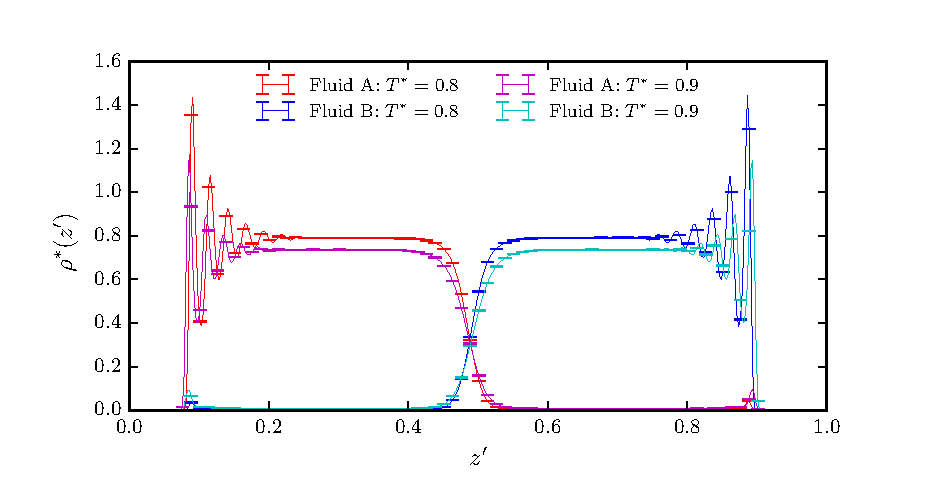
\includegraphics[scale=1.0]{PisVirRho}
\caption{The number density for the two fluids confined between two walls at $T^{*} = 0.8$ and $T^{*} = 0.9$ was time--averaged over $40 \times 10^{6}$ timesteps of length $0.001\ \tau$. 
The bulk density is uniform, representing a fluid state, and the interface manifests itself as a sharp change in the densities of the two fluids.
Structural layering of the fluid creates oscillations in the density close to the walls.
}
\label{PisVirRho}
\end{figure*}

\begin{figure*}[h!]
\centering
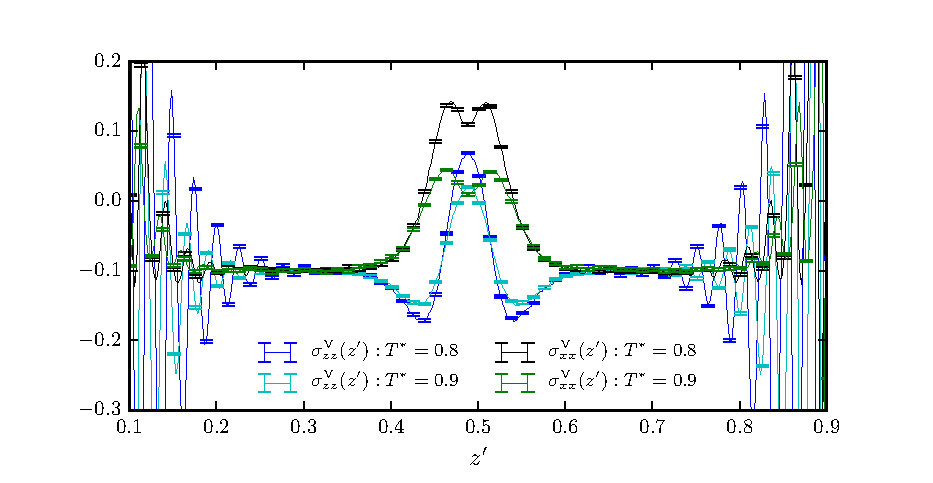
\includegraphics[scale=1.0]{PisVirStress}
\caption{The virial stress tensor components for the combined fluid confined between two walls at $T^{*} = 0.8$ and $T^{*} = 0.9$ were time--averaged over $40 \times 10^{6}$ timesteps of length $0.001\ \tau$.
Both the normal and tangential stress show bulk values equal to $-P_{ext}$, representing the hydrostatic pressure.
There is a peak in the tangential stress at the interface due to the anisotropy of the interparticle forces in this region.
This can be related to the surface tension and its temperature dependence is the driving force for the Marangoni effect.
There is also a change in the normal component at the interface, resulting from the dependence of the virial stress on density deviations.
Towards the wall there are temperature dependent oscillations in both components, providing the origin of the thermophoretic force.
}
\label{PisVirStress}
\end{figure*}

Both the density and stress profiles show the characteristics expected of a binary--mixture. 
The bulk density is uniform density and there is an interfacial region of where the density of one species falls sharply and the density of the other increases.
Close to the walls, there are density oscillations resulting from structural layering of the fluid.

The bulk values for the normal and tangential stress components are equal to $-P_{\mathrm{ext}}$, corresponding to the hydrostatic fluid pressure as expected.
There is an interfacial peak in the tangential stress due to the anisotropy of the intermolecular forces in this region; this is related to the interfacial tension.\cite{Marchand2011}
Furthermore, the normal component changes at the interface, resulting from the dependence of the virial stress on density deviations in this region.

The time--averaged values for the stress were then used to estimate the temperature derivative of the tangential stress through Equation \ref{FinDiff}, as shown in Figure \ref{PisVirForce}.
This derivative shows a peak at the interface, providing the origin of the Marangoni force.
In the bulk of the fluid the derivative is zero within statistical error, ensuring no force acts this region.
In addition, the derivative oscillates at the surface of the wall.
This can be interpreted as a thermophoretic force and is henceforth ignored.

\begin{figure*}[h!]
\centering
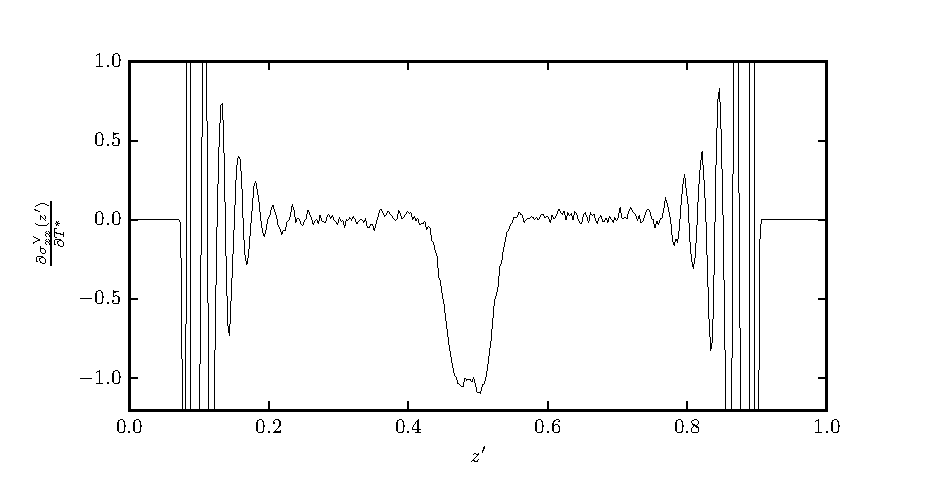
\includegraphics[scale=1.0]{PisVirForce}
\caption{The derivate of the tangential component of the virial stress with respect to temperature was calculated using the finite difference approximation.
This shows a negative peak in the interfacial region.
When combined with a specified temperature gradient, a force in the opposite direction to a temperature gradient is generated, imitating the Marangoni force.
The oscillations at the liquid--solid surface create the thermophoretic force and are subsequently ignored.}
\label{PisVirForce}
\end{figure*}
\FloatBarrier

Using the central $1/3$ of the derivative profile and a temperature gradient of $\partial T^{*} / \partial x^{*} = 0.001$, an artificial Marangoni force was computed through Equation \ref{ForceStressTemp}.
This force was applied to an identical system prepared at $T^{*} = 0.85$.
An equilibrium simulation was then run for $40 \times 10^{6}$ timesteps, and the time--average of the x--component of the fluid velocity $v^{*}_{x}(z')$ was computed.
The momenta of the walls in the $x,y$ plane were fixed to provide a stationary reference point, creating a momentum sink.

\begin{figure*}[h!]
\centering
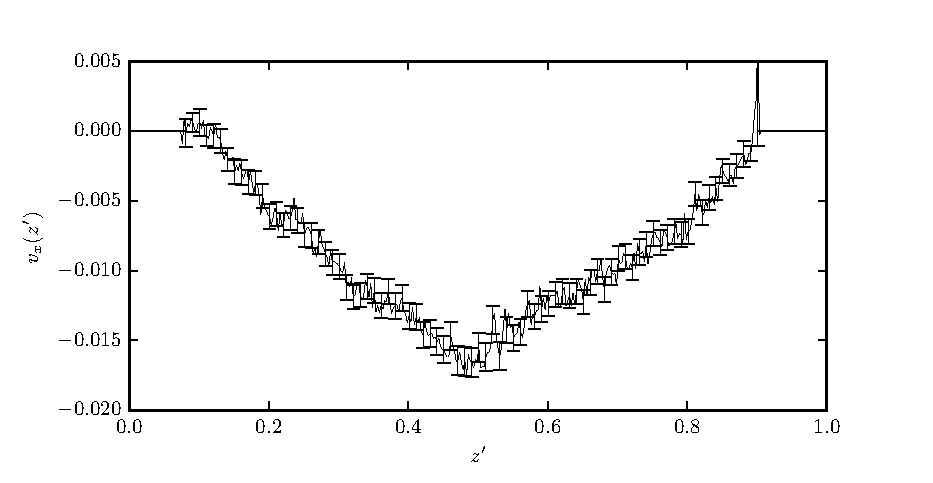
\includegraphics[scale=1.0]{PisVirFlow}
\caption{The velocity profile of a confined fluid at $T^{*}=0.85$ with an applied force calculated from Figure \ref{PisVirForce} was time--averaged over $40 \times 10^{6}$ timesteps of length $0.001\ \tau$.
A steady state negative interfacial peak emerges, corresponding to a Marangoni flow in the opposite direction to the temperature gradient.
The magnitude of the peak velocity is approximately 0.16 and this decays linearly to zero at the surface of the bounding walls, corresponding to a Couette flow.}
\label{PisVirFlow}
\end{figure*}
The velocity profile is shown in Figure \ref{PisVirFlow}. 
There is a sharp negative peak at the interface indicating a Marangoni flow in the opposite direction to the temperature gradient.
Furthermore, the flow decays linearly away from the interface, consistent with a Couette flow arising from shear--driven fluid motion.\cite{FluidMech}

There is also a net flow in the system, suggesting an overall force acting on the fluid.
The walls provide a frictional force which allows this steady--state flow to arise under the isolated effect of a temperature--gradient.
\FloatBarrier

\subsubsection{Comparing to the Irving--Kirkwood stress}
Figure \ref{PisVirStress} shows the normal component of the virial stress is not uniform across the interface.
In contrast, the normal component of the Irving--Kirkwood stress does not depend on the local fluid density and should be constant throughout the liquid.
To verify if the difference in these methods is significant for the measurement of Marangoni forces, the Irving--Kirkwood stress was also calculated.

\begin{figure*}[h!]
\centering
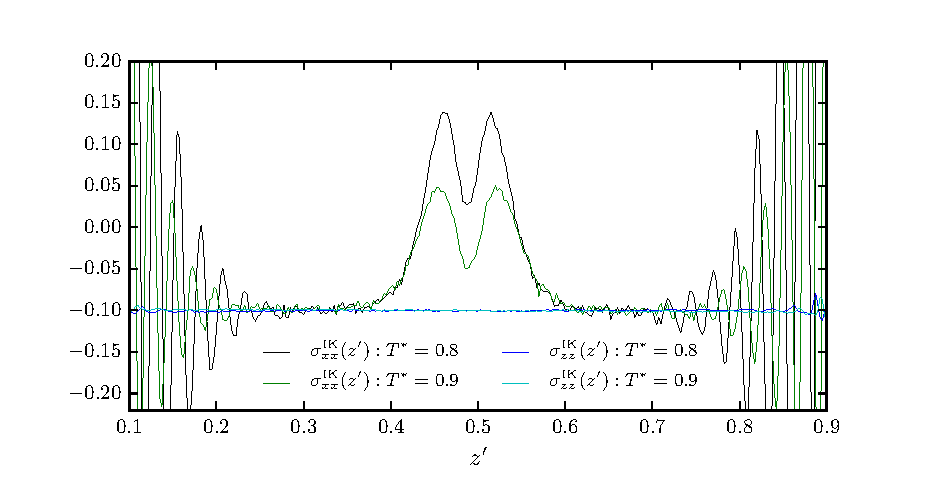
\includegraphics[scale=1.0]{PisIKStress}
\caption{The Irving--Kirkwood stress tensor components for the combined fluid confined between two walls at $T^{*} = 0.8$ and $T^{*} = 0.9$ were time--averaged over $1 \times 10^{6}$ timesteps of length $0.001\ \tau$.
Both the normal and tangential stress show bulk values equal to $-P_{ext}$, representing the hydrostatic pressure.
Similar to Figure \ref{PisVirStress}, there is a peak in the tangential stress at the interface due to the anisotropy of the interparticle forces in this region.
However, this peak is divided into two with a reduction in the stress directly at the interface.
This difference to the virial stress arises because the Irving--Kirkwood stress does not depend on the local density. 
The normal components of the stress are constant across the system, as expected.
}
\label{PisIKStress}
\end{figure*}
\FloatBarrier 
The fluids were prepared at $P^{*}=0.1$ and $T^{*}=0.8$ and $T^{*}=0.9$ as before.
Since the Irving--Kirkwood stress tensor was more computationally expensive (see Section \ref{CalcStress}), the equilibrium simulations were only run for $1 \times 10^{6}$ timesteps, resulting in a greater amount of statistical error.
The time--averaged stress is plotted in Figure \ref{PisIKStress}.
The tangential component shows a similar profile to the virial stress, although the interfacial peak is divided into two with a reduction in the stress directly at the interface.
This difference directly at the interface arises since the Irving--Kirkwood does not depend on local density.
The normal component of the Irving--Kirkwood stress is uniform, representing the isotropy of the system in this direction.
\FloatBarrier

\begin{figure*}[h!]
\centering
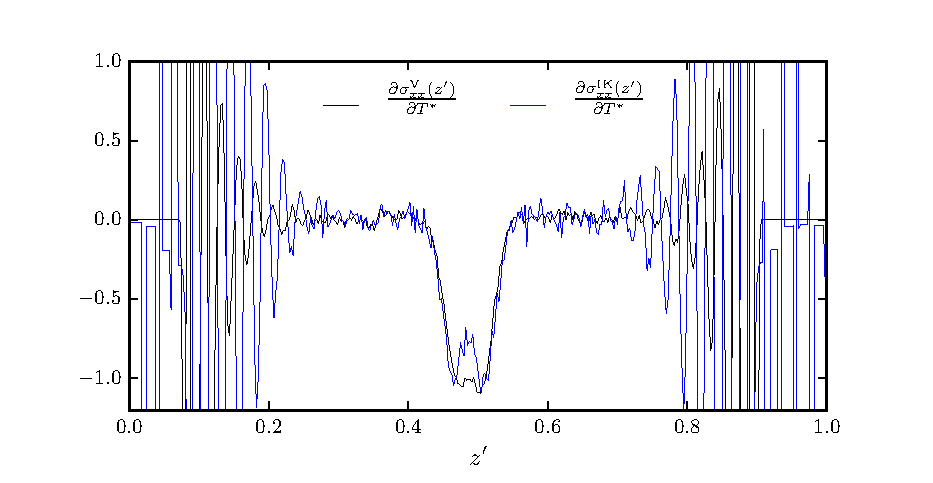
\includegraphics[scale=1.0]{PisIKForce}
\caption{The derivate of the tangential component of the Irving--Kirkwood stress with respect to temperature was calculated using the finite difference approximation.
There is an analogous negative peak in the interfacial region to Figure \ref{PisVirForce}, with a similar magnitude and spatial extent.
However, the peak in the Irving--Kirkwood derivative is split into two.
This difference arises because, unlike the virial stress, the Irving--Kirkwood stress does not depend on local density.
When combined with a specified temperature gradient, a force in the opposite direction to a temperature gradient is generated, imitating the Marangoni force.
The derivative in the bulk is zero, providing no body force acting on the fluid away from the interface.
}
\label{PisIKForce}
\end{figure*}
The finite difference method was again used to calculate the temperature derivative of the stress, and this is compared to the virial result in Figure \ref{PisIKForce}.
Still focussing on the central $1/3$ of the fluid, there is a good correspondence between the two derivatives and the interfacial peak occurs across the same spatial region and with the same maximum value.
The most significant difference appears directly at the interface, where there is a sharp reduction in the derivative of the Irving--Kirkwood stress.
This is probably a result of the reduction in density at the interface affecting the virial and not the Irving--Kirkwood stress.
\FloatBarrier

\begin{figure*}[h!]
\centering
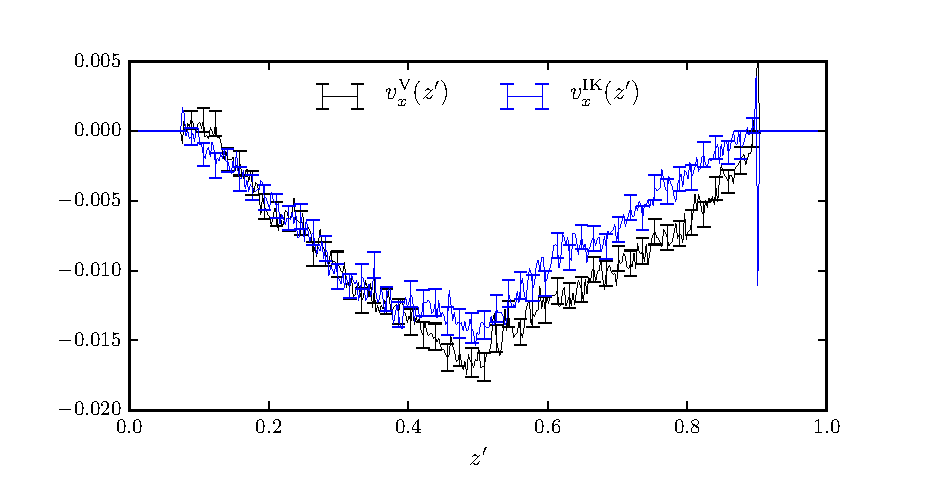
\includegraphics[scale=1.0]{PisIKFlow}
\caption{The velocity profile of a confined fluid at $T^{*}=0.85$ with an applied force calculated from Figure \ref{PisIKForce} was time--averaged over $40 \times 10^{6}$ timesteps of length $0.001\ \tau$.
This is compared to the velocity profile produced using the force calculated from the virial stress.
Both show a steady state negative interfacial peak, corresponding to a Marangoni flow in the opposite direction to the temperature gradient, with a linear decay into the bulk.
The peak value using the force calculated from the Irving--Kirkwood stress is not as large as that using the force calculated from the virial stress.
This is a result of the reduction of the Irving--Kirkwood stress derivative directly at the interface.
Moreover, the virial flow is symmetric about the interface whilst the Irving--Kirkwood flow is not. 
This is probably a result of the increase in noise in the Irving--Kirkwood derivative due to a shorter simulation time.}
\label{PisIKFlow}
\end{figure*}
Using a temperature gradient of $\partial T^{*} / \partial x^{*} = 0.001$ to compute the Irving--Kirkwood artificial body force, an equilibrium simulation at $T^{*} = 0.85$ was run for $40 \times 10^{6}$ timesteps.
The fluid velocity was measured and compared to the result obtained using the virial force, as shown in Figure \ref{PisIKFlow}.
The profiles show a close correspondence, especially for the region $z' \leq 0.4$, although they deviate for higher values of $z'$.
In particular, the flow from the Irving--Kirkwood method is smaller directly at the interface, due to the reduction in the force at this point.
The Irving--Kirkwood velocity is also asymmetric despite the symmetry of the system.
This may be the result of the increased noise in the Irving--Kirkwood force relative to the virial force, resulting from the shorter simulation time enforced by the high computational cost of the Irving--Kirkwood analysis.

\FloatBarrier
\subsection{Binary--mixture periodic in 3-dimensions}
Equation \ref{NavierStokes} demonstrated that a temperature gradient in a system cannot generate a net fluid flow.
Levich described how the interfacial flow must be accompanied by a back--flow in the bulk.\cite{Levich}
For the binary--mixture held between two walls, the walls provide a momentum sink allowing a net flow to exist within the fluid.
To replicate the behaviour of an infinite fluid where a back flow may be observed, a system void of momentum sinks must be studied.
For example, a binary--mixture of two partially miscible fluids with periodic boundary conditions in all dimensions can be used.

This system, shown in Figure \ref{AABB}, was prepared as described in Section \ref{SystemPrep} with the parameters given in Section \ref{InteractionModel}.
The distance between consecutive interfaces was $0.5 L_{z^{*}}$.
A Nos\'{e}--Hoover barostat and thermostat were used to regulate the pressure at $P^{*} = 0.1$ with temperatures of $T^{*}=0.8$ and $T^{*}=0.9$.

\subsubsection{Comparing the virial and Irving--Kirkwood stress}
Again there is an ambiguity over which stress tensor should be used to compute the Marangoni force.
Once equilibrated, the system was simulated for $10 \times 10^{6}$ timesteps over which the number density, virial and Irving--Kirkwood stress were computed.
The Irving--Kirkwood analysis was computationally expensive and this was the longest feasible simulation length.
\FloatBarrier

\begin{figure}[h!]
\centering
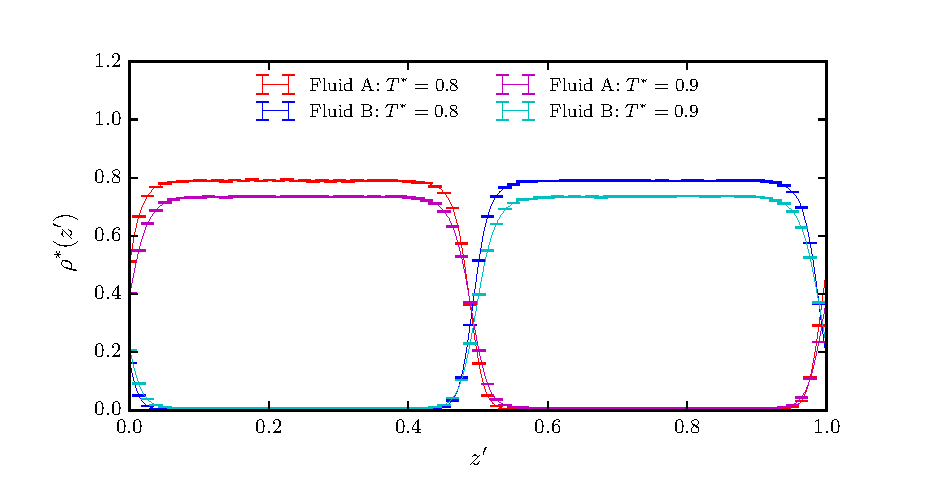
\includegraphics[scale=1.0]{Period10Rho}
\caption{The number density for the two fluids periodic in all dimensions at $T^{*} = 0.8$ and $T^{*} = 0.9$ was time--averaged over $10 \times 10^{6}$ timesteps of length $0.001\ \tau$. 
The bulk density is uniform, representing a fluid state, and the interfaces manifest themselves as a sharp change in the densities of the two fluids.
Between the two temperatures the position of the interface is slightly shifted, this must be corrected before calculating the stress derivative.
}
\label{Period10Rho}
\end{figure}
The resulting density profile plotted in Figure \ref{Period10Rho} showed a uniform bulk density and a sharp interfacial region as expected.
However, the position of the interface shifted during the simulation and was no longer coincident for the two temperatures.
Recentering the interfaces removed this shift before calculating the Marangoni force.
\FloatBarrier

\begin{figure}[h!]
\centering
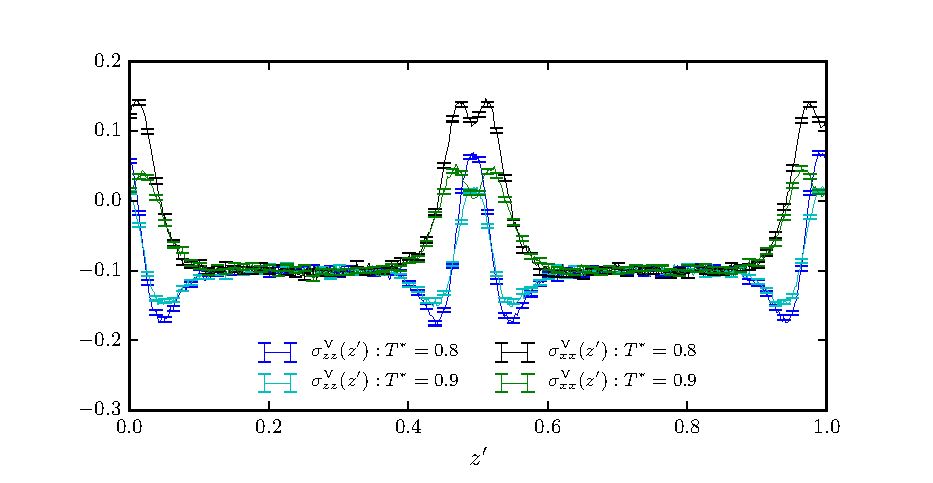
\includegraphics[scale=1.0]{Period10VirStress}
\caption{The virial stress tensor components for the combined fluid periodic in all dimensions $T^{*} = 0.8$ and $T^{*} = 0.9$ were time--averaged over $10 \times 10^{6}$ timesteps of length $0.001\ \tau$.
Both the normal and tangential stress show bulk values equal to $-P_{ext}$, representing the hydrostatic pressure.
There is a peak in the tangential stress at the interface due to the anisotropy of the interparticle forces in this region.
This peak has a similar form to that seen in Figure \ref{PisVirStress}, and its temperature dependence provides the origin of the Marangoni effect.
There is also a change in the normal component at the interface, resulting from the dependence of the virial stress on density deviations.
}
\label{Period10VirStress}
\end{figure}

\begin{figure}[h!]
\centering
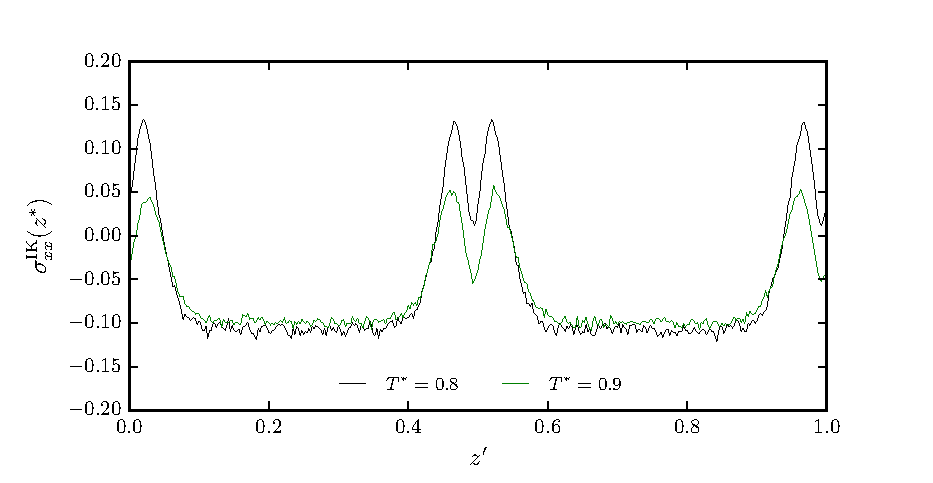
\includegraphics[scale=1.0]{Period10IKStress}
\caption{The Irving--Kirkwood stress tensor components for the combined fluid periodic in all dimensions $T^{*} = 0.8$ and $T^{*} = 0.9$ were time--averaged over $10 \times 10^{6}$ timesteps of length $0.001\ \tau$.
Both the normal and tangential stress show bulk values equal to $-P_{ext}$, representing the hydrostatic pressure.
There is a peak in the tangential stress at the interface due to the anisotropy of the interparticle forces in this region.
This peak has a similar form to that seen in the virial stress, although they deviate directly at the interface.
Since the Irving--Kirkwood stress does not depend on local density, the normal component is uniform across the system, as expected.
}
\label{Period10IKStress}
\end{figure}
The recentered virial and Irving--Kirkwood stress components are plotted in Figures \ref{Period10VirStress} and \ref{Period10IKStress} respectively.
As with the confined fluid, the bulk stress components are equal to $-P_{\mathrm{ext}}$, corresponding to the hydrostatic fluid pressure.
There is an interfacial peak in both the virial and Irving--Kirkwood tangential stress at the interface with a similar maximum value, although the Irving--Kirkwood stress shows a stronger minimum directly at the interface.
Similar to Figure \ref{PisIKStress}, this is probably the result of a reduced density in the interfacial region.
Furthermore, the normal component of the Irving--Kirkwood stress is uniform across the interface, as expected.

\FloatBarrier
The temperature derivative of the tangential stress was calculated through the finite difference approach.
The derivative profile was adjusted by subtracting the average from each value, ensuring the integral over all space was zero, as shown in Figure \ref{Period10Force}.
This guaranteed there would be no net force applied to the fluid, even in the absence of a momentum sink.

\begin{figure}[h!]
\centering
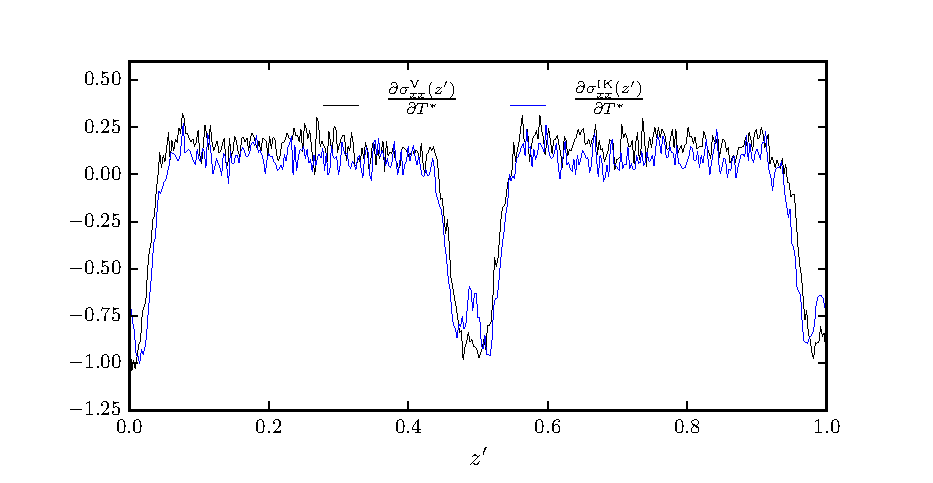
\includegraphics[scale=1.0]{Period10Force}
\caption{The derivate of the tangential component of the Irving--Kirkwood and virial stress with respect to temperature was calculated using the finite difference approximation.
The average value was subtracted to ensure the integral of the derivative profile over all space was zero.
Both the virial and Irving--Kirkwood stress derivatives show a negative peak at the interface, with a similar maximum value and spatial extent.
However, there is too much noise in these profiles, obscuring the fine structure and preventing a definitive comparison.
Furthermore, these derivatives are not precise enough to be useful for calculating an artificial body force.
}
\label{Period10Force}
\end{figure}
The derivative profile shows a similar interfacial peak to Figure \ref{PisIKForce}. 
The maximum values are similar, suggesting that fixing the total force to zero correctly adjusts the derivatives to give a physically meaningful Marangoni force.
There is a good correspondence between the derivatives calculated from the Irving--Kirkwood and virial stress tensors, although the magnitude of the Irving--Kirkwood peak is reduced directly at the interface.
In the bulk fluid, the derivative opposes the interfacial peak, generating the back force which balances the Marangoni force.
However, the profile shows too much noise for determination of the fine--structure and is not of sufficient quality for calculating an artificial body--force.

\subsubsection{Reducing the noise in the force--profile}
To generate a profile with reduced noise requires either a larger system or a longer simulation time.
Both of these increase the computational cost of calculating the Irving--Kirkwood stress beyond a practical level, and only the virial stress can be used.
Considering how similar the virial and Irving--Kirkwood derivative profiles appear in Figure \ref{PisIKForce}, using the virial stress does not create too much deviation from the more suitable Irving--Kirkwood stress, whilst enabling a much longer simulation time.
\FloatBarrier

\begin{figure}[h!]
\centering
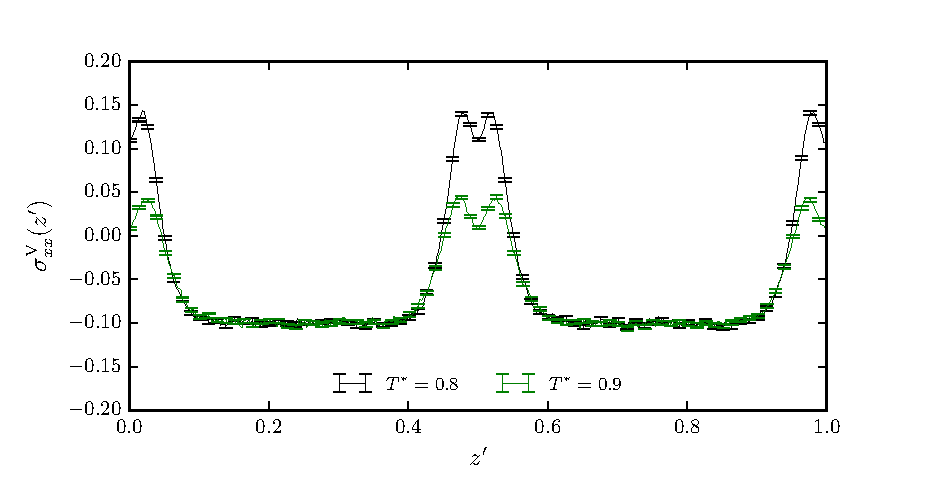
\includegraphics[scale=1.0]{Period30VirStress}
\caption{The virial stress tensor components for the combined fluid periodic in all dimensions $T^{*} = 0.8$ and $T^{*} = 0.9$ were time--averaged over $30 \times 10^{6}$ timesteps of length $0.001\ \tau$.
This produced a significant reduction in noise relative to Figure \ref{Period10VirStress}.
As before, both the normal and tangential stress show bulk values equal to $-P_{ext}$, representing the hydrostatic pressure.
There is a peak in the tangential stress at the interface due to the anisotropy of the interparticle forces in this region.
The normal component at the interface also deviates from the bulk value as a result of the dependence of the virial stress on the local density.
}
\label{Period30VirStress}
\end{figure}

The reduced noise stress was calculated by running the equilibrium systems for $30 \times 10^{6}$ timesteps.
Recentering the interfaces generated the virial stress shown in Figure \ref{Period30VirStress}.
For both temperatures, the profiles show much less noise compared to Figure \ref{Period10VirStress}, especially in the bulk region, and the interfacial peaks are more symmetric.
\FloatBarrier

\begin{figure}[h!]
\centering
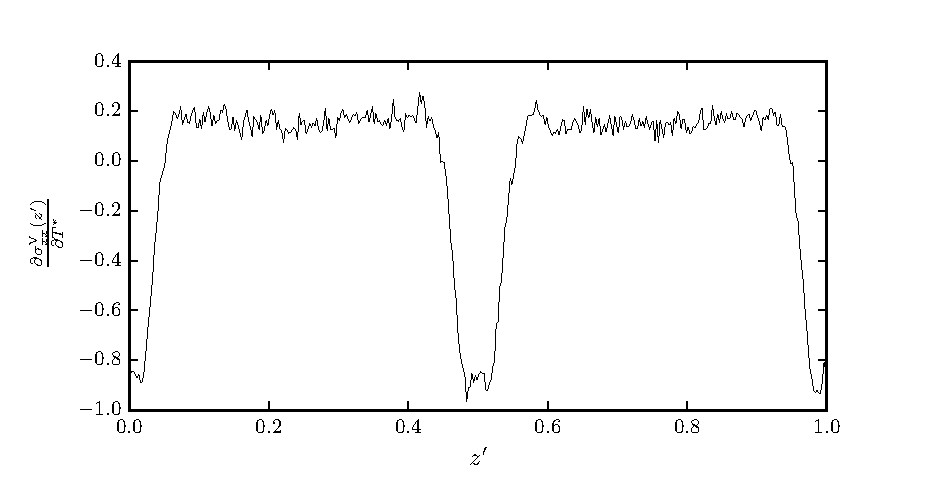
\includegraphics[scale=1.0]{Period30VirForce}
\caption{The derivate of the tangential component of the virial stress was calculated using the finite difference approach.
The average value was subtracted to ensure the integral of the derivative profile over all space was zero.
There is a significant reduction in noise compared to Figure \ref{Period10Force}.
A sharp, negative peak can be seen at the interface, leading to the Marangoni force, and an opposing derivate occurs in the bulk of the fluid, yielding a balancing back flow.
}
\label{Period30VirForce}
\end{figure}

The temperature derivative of the tangential stress was again computed using the finite difference and the average value subtracted to give the profile shown in Figure \ref{Period30VirForce}.
There is a dramatic reduction in the noise compared to Figure \ref{Period10Force}, with a peak at the interface and an opposing derivative in the bulk regions.
\FloatBarrier

Using the stress derivative given in Figure \ref{Period30VirForce} and a temperature gradient of $\partial T^{*} / \partial x^{*} = 0.001$, an artificial body force was computed.
This force was applied in an equilibrium simulation at $T^{*} = 0.85$ and run for $40 \times 10^{6}$ timesteps.
The time--averaged velocity $v^{*}_x(z')$ was computed to give the profile plotted in Figure \ref{Period30VirFlow}.

\begin{figure}[h!]
\centering
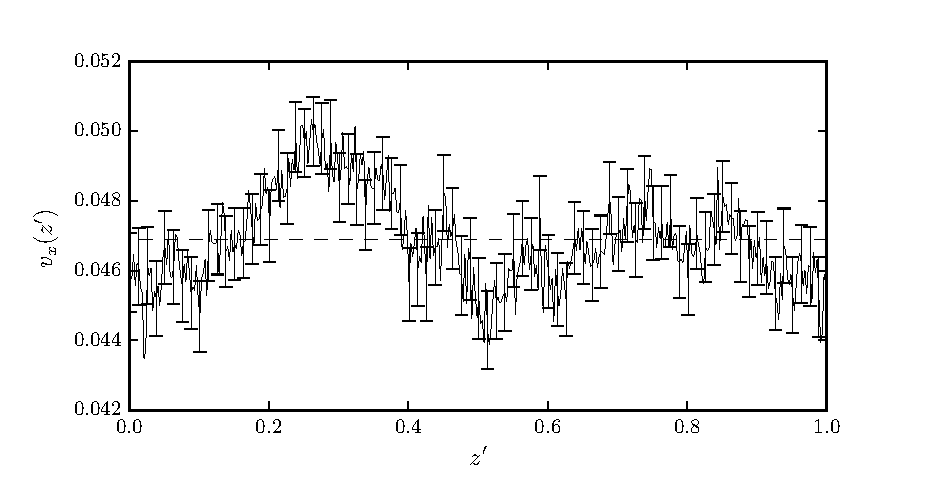
\includegraphics[scale=1.0]{Period30VirFlow}
\caption{The velocity profile of an infinite binary--mixture at $T^{*}=0.85$, with an applied force calculated using Figure \ref{Period30VirForce} and temperature gradient of $\partial T^{*} / \partial x^{*} = 0.001$, was time--averaged over $40 \times 10^{6}$ timesteps of length $0.001\ \tau$.
A non--equilibrium emerges with a non--zero average velocity (indicated by the hashed line), despite the average derivative being fixed to zero.
It is unlikely this could be removed without artificially fixing the centre--of--mass.
Despite this, the fluid velocity relative to this centre--of--mass motion suggests a Marangoni flow at the interfaces with an opposing flow in the bulk regions, as predicted by Levich.\cite{Levich}
}
\label{Period30VirFlow}
\end{figure}

% Need to decide how to discuss this figure, possibly waiting on results from current simulations.
Despite the simulation being run for a long timescale, the velocity profile still retains a lot of statistical noise.
It would be difficult practically to reduce this noise further.
Moreover, the average velocity (indicated by the hashed line) is non--zero, indicating centre--of--mass motion during the simulation.
This motion occurs even though the stress derivative has been adjusted to give no net force overall.
It is likely that in the absence of a momentum sink for a system like this, it would be very difficult to completely remove this net flow without artificially fixing the centre--of--mass throughout the simulation.

Despite this, the relative motion across the fluid can still be considered, and there does appear to be a velocity peak at the interface (with $v < v_{\mathrm{COM}}$), corresponding to a Marangoni flow, with a back flow in the bulk fluid (with $v > v_{\mathrm{COM}}$) as predicted.
This result is, however, somewhat ambiguous and there was insufficient time to improve this simulation further.

\subsection{The effect of surfactants}\label{SurfResult}
Surfactant molecules decrease surface tension as they have a favourable interaction with both fluids and bridge the interfacial plane.
This should also decrease a surface tension gradient and reduce the Marangoni effect, as observed experimentally.\cite{KimSubramanianA,KimSubramanianB,BartonSubramanian,ChenStebe}

The non--ionic surfactant molecules described in Section \ref{ModellingSurfactants} were added to the binary--mixture confined between two walls.
This system was chosen since Section \ref{Piston} showed it allowed a steady--state flow to be modelled effectively.

The surfactant molecules were added to a single plane between the two fluids in the initial lattice before melting.
A certain fraction of these molecules were then removed to vary the surfactant concentration, quantified as a fraction of the total number of particles present,
\begin{equation}
\mathrm{Surfactant\ Fraction} \equiv \frac{N_{\mathrm{surfactant}}}{N_{\mathrm{surfactant}}+N_{\mathrm{fluid}}}.
\end{equation}
This allowed the surfactant fraction to be varied between $0$ and $0.0323$.

Taking fractions of $0.000$, $0.0031$, $0.0098$, $0.0194$, $0.0264$, $0.0298$ and $0.0323$, the fluid was prepared as described in Section \ref{SystemPrep}, with a pressure of $P^{*}=0.1$ and temperatures of $T^{*}=0.8$ and $T^{*}=0.9$.
A piston barostat and Nos\'{e}--Hoover thermostat were used and each system was run at equilibrium for $30 \times 10^{6}$ timesteps of length $0.001\ \tau$.

\begin{figure}[h!]
\centering
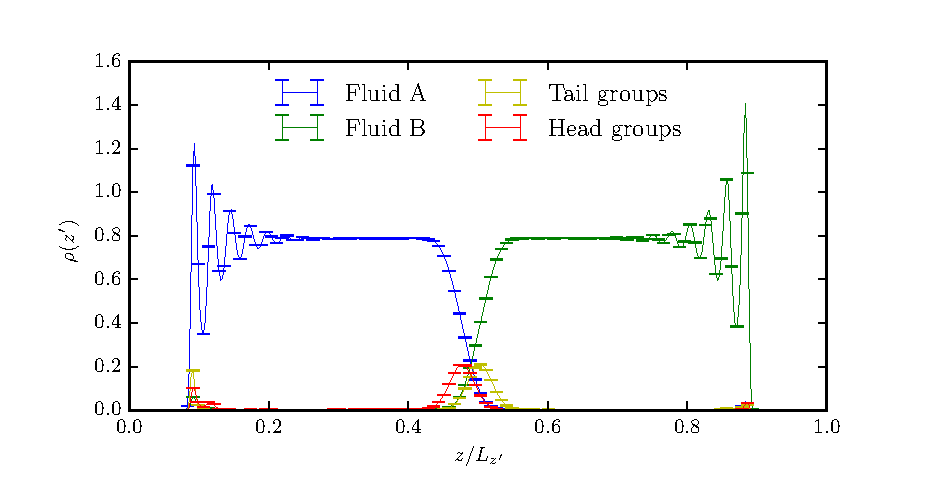
\includegraphics[scale=1.0]{SurfRho}
\caption{The number density for the confined binary--mixture with a non--ionic surfactant fraction of $0.0194$, pressure of $P^{*}=0.1$ and at $T^{*}=0.8$ was time--averaged over $30 \times 10^{6}$ timesteps of length $0.001\ \tau$. 
There is a uniform density in the bulk, and an interface represented by a sharp change in the densities of Fluid A and Fluid B.
The surfactant particles are localised at the interface with a low solubility.
They show the correct orientation, with `Head' particles interacting most strongly with Fluid A and `Tail' particles with Fluid B.
}
\label{SurfRho}
\end{figure}

The number density of each species shows a uniform bulk density, a sharp interface and peaks for the head and tail groups located at the interface, as shown for $T^{*}=0.8$ and a surfactant fraction of $0.0194$ in Figure \ref{SurfRho}.
The surfactant molecules were correctly oriented with head groups interacting with Fluid A and tail groups with Fluid B.
\FloatBarrier

\begin{figure}[h!]
\centering
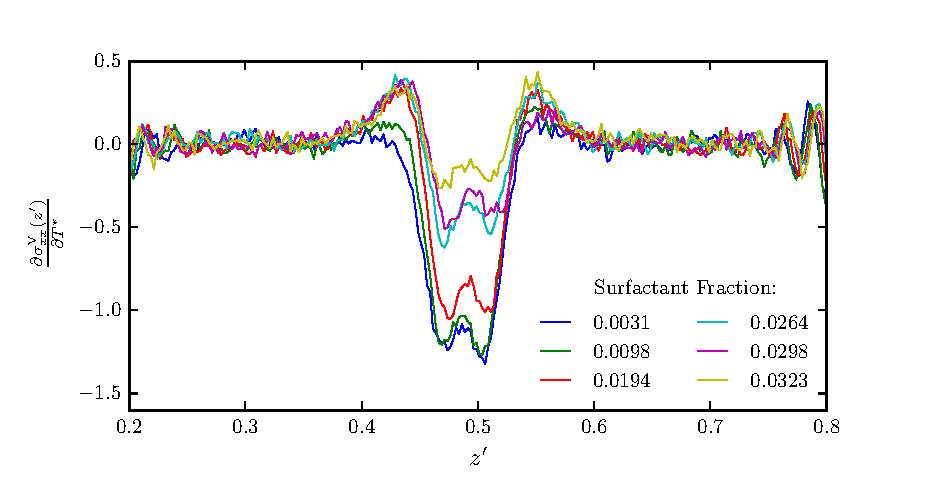
\includegraphics[scale=1.0]{SurfForce}
\caption{The derivative of the tangential component of the virial stress with respect to temperature was calculated for a range of surfactant fractions using the finite difference approximation.
For a low surfactant fraction, there is strong interfacial peak providing the origin of the Marangoni force.
As the amount of surfactant is increased, the strength of this peak decreases to zero indicating the eradication of the Marangoni effect.
Two smaller positive peaks on either side of the centre also develop for higher surfactant fractions.
This probably results from an increase in the number density in this region, due to localisation of the surfactant particles at the interface.
}
\label{SurfForce}
\end{figure}

The virial stress was computed used to compute the temperature derivative of the tangential stress for each surfactant fraction.
These results, plotted in Figure \ref{SurfForce}, show a reduction in the magnitude of the interfacial peak as the surfactant fraction increases, corresponding to a reduction in the Marangoni force.

Two smaller positive peaks on either side of the centre also develop for higher surfactant fractions.
These may be the result of an increase in the local density, due to localisation of the surfactant particles in this region and the density dependence of the virial stress.
An increase in surfactant fraction would exaggerate this density change.
This could be verified by computing the Irving--Kirkwood stress, where any peaks due to density deviations should disappear.

Furthermore, the harmonic forces in the surfactant molecules could contribute to these peaks.
This could be investigated by varying the spring constant for the surfactant bond.
\FloatBarrier

\begin{figure}[h!]
\centering
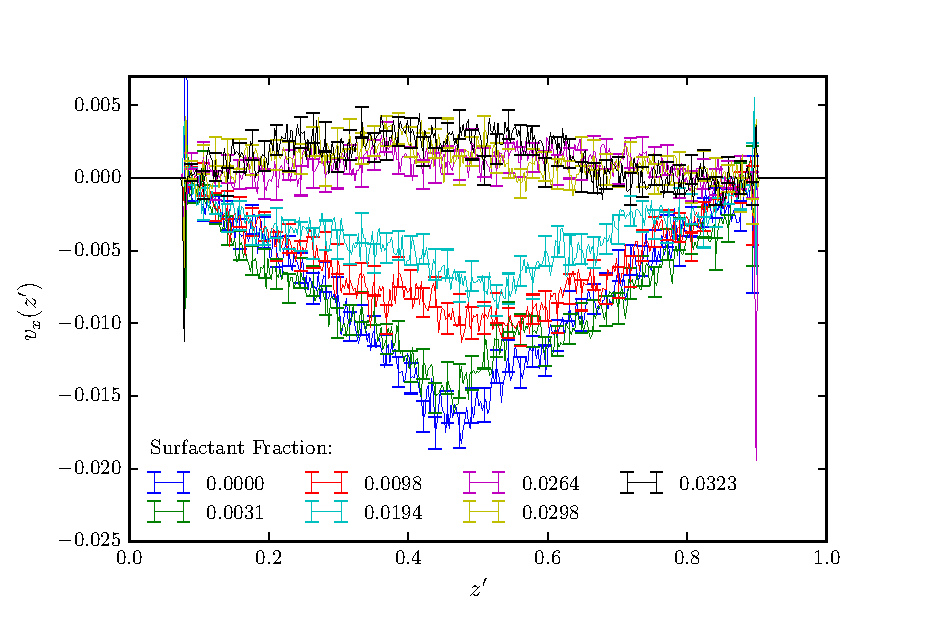
\includegraphics[scale=1.0]{SurfFlow}
\caption{The velocity profile of an confined binary--mixture at $T^{*}=0.85$, with an applied force calculated using Figure \ref{SurfForce} and temperature gradient of $\partial T^{*} / \partial x^{*} = 0.001$, was time--averaged over $40 \times 10^{6}$ timesteps of length $0.001\ \tau$ for a range of surfactant fractions.
For a low surfactant fraction, the flow profile closely resembles that of the non--surfactant system (Figure \ref{PisVirFlow}, with a negative interfacial peak and a linear decay into the bulk.
As the amount of surfactant increases there is a reduction in the magnitude of this peak until the Marangoni flow essentially disappears.
Moreover, the peak becomes less sharp at higher surfactant fractions.
This is probably due to the non--uniform viscosity created by the added surfactant molecules.
}
\label{SurfFlow}
\end{figure}
Using a temperature gradient of $\partial T^{*} / \partial x^{*} = 0.001$, the central $1/3$ of the stress derivative profiles in Figure \ref{SurfForce} were used to compute an artificial body force, which was applied to simulations at $T^{*}=0.85$.
These were run for $30 \times 10^{6}$ timesteps over which $v_{x}(z')$ was measured and plotted in Figure \ref{SurfFlow}.
The interfacial velocity decreases as the surfactant fraction is increased, suggesting a surfactant induced retardation of the Marangoni flow.

\FloatBarrier
\begin{figure}[h!]
\centering
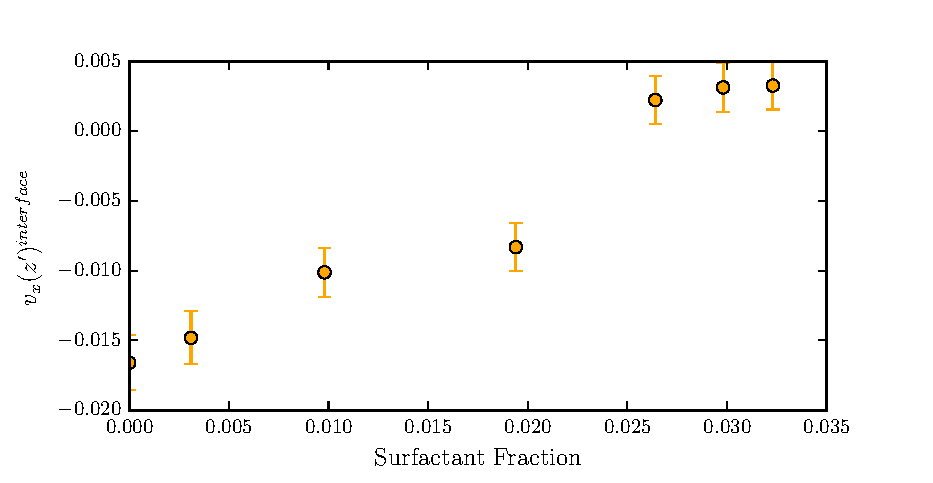
\includegraphics[scale=1.0]{InterVel}
\caption{Comparing the surfactant fraction to the interfacial velocity demonstrates the retardation of the Marangoni flow in the presence of surfactant molecules.
Above a fraction of $0.025$, this velocity is essentially zero, although there is small velocity in the opposite direction to the Marangoni flow.
This may be the result of the secondary peaks that emerge in Figure \ref{SurfForce} which only become significant for high surfactant fractions.
}
\label{InterVel}
\end{figure}
Comparing the peak value of the flow velocity against the surfactant fraction shows a reduction in the peak magnitude as the surfactant fraction increases, as shown in Figure \ref{InterVel}.
Above a fraction of $0.025$ the Marangoni effect has effectively been removed.
This retardation has been observed experimentally by Barton and Subramanian, and is discussed in their study on the relation between droplet size and motion under a vertical  temperature gradient.\cite{BartonSubramanian} 
They note that droplets sink on the addition of a non--ionic surfactant, indicating the eradication of the Marangoni force and the dominance of gravity.

\FloatBarrier
The sharpness of the Marangoni flow peak in Figure \ref{SurfFlow} also decreases as the surfactant fraction increases and no longer fits the Couette model as conclusively.
This may be due to a reduction in viscosity at the interface from the presence of surfactant molecules, giving a non-uniform viscosity across the fluid. 
To confirm this, the viscosity could be measured using the Green--Kubo relation,
\begin{equation}
\eta = \frac{1}{V k_{\mathrm{B}} T} \int_{0}^{\infty} \left< \sigma_{xy} \left( \tau \right) \sigma_{xy}(0) \right> \mathrm{d} \tau.
\end{equation}
